% The groups of order 1 to 15 up to isomorphism (Z_n stands for Z/nZ): abelian ones in blue, non-abelian in orange, with the reason. Generated by a short script.
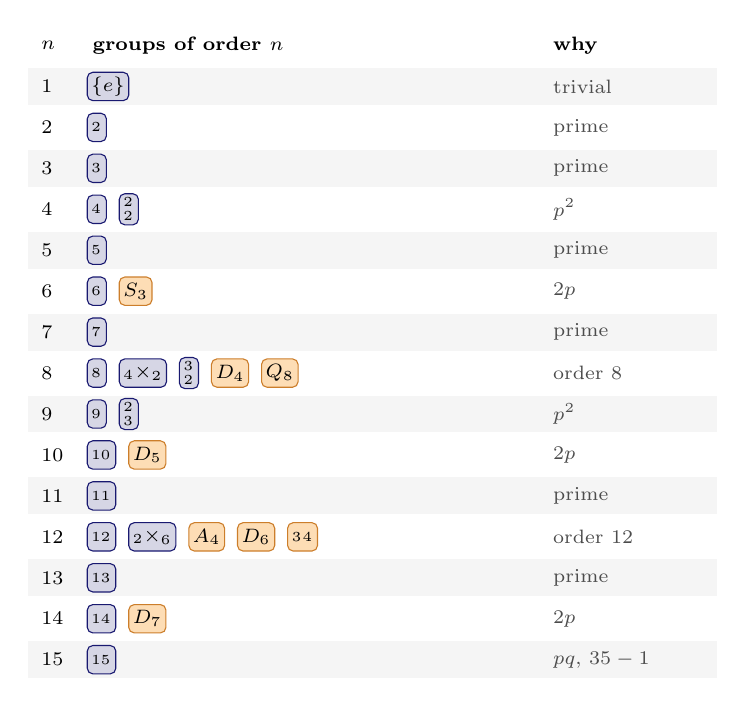
\begin{tikzpicture}[x=1cm,y=0.52cm]
\node[font=\scriptsize\bfseries,anchor=west] at (-0.1,1) {$n$};
\node[font=\scriptsize\bfseries,anchor=west] at (0.55,1) {groups of order $n$};
\node[font=\scriptsize\bfseries,anchor=west] at (6.4,1) {why};
\fill[black!4] (-0.15,-0.45) rectangle (8.6,0.45);
\node[font=\scriptsize,anchor=west] at (-0.1,0) {$1$};
\node[font=\scriptsize,anchor=west,fill=MidnightBlue!18,draw=MidnightBlue,rounded corners=2pt,inner sep=1.5pt,minimum height=0.36cm] (g1x0) at (0.6,0) {$\{e\}$};
\node[font=\scriptsize,anchor=west,text=black!70] at (6.4,0) {trivial};
\node[font=\scriptsize,anchor=west] at (-0.1,-1) {$2$};
\node[font=\scriptsize,anchor=west,fill=MidnightBlue!18,draw=MidnightBlue,rounded corners=2pt,inner sep=1.5pt,minimum height=0.36cm] (g2x0) at (0.6,-1) {$\Z_2$};
\node[font=\scriptsize,anchor=west,text=black!70] at (6.4,-1) {prime};
\fill[black!4] (-0.15,-2.45) rectangle (8.6,-1.55);
\node[font=\scriptsize,anchor=west] at (-0.1,-2) {$3$};
\node[font=\scriptsize,anchor=west,fill=MidnightBlue!18,draw=MidnightBlue,rounded corners=2pt,inner sep=1.5pt,minimum height=0.36cm] (g3x0) at (0.6,-2) {$\Z_3$};
\node[font=\scriptsize,anchor=west,text=black!70] at (6.4,-2) {prime};
\node[font=\scriptsize,anchor=west] at (-0.1,-3) {$4$};
\node[font=\scriptsize,anchor=west,fill=MidnightBlue!18,draw=MidnightBlue,rounded corners=2pt,inner sep=1.5pt,minimum height=0.36cm] (g4x0) at (0.6,-3) {$\Z_4$};
\node[font=\scriptsize,anchor=west,xshift=0.15cm,fill=MidnightBlue!18,draw=MidnightBlue,rounded corners=2pt,inner sep=1.5pt,minimum height=0.36cm] (g4x1) at (g4x0.east) {$\Z_2^2$};
\node[font=\scriptsize,anchor=west,text=black!70] at (6.4,-3) {$p^2$};
\fill[black!4] (-0.15,-4.45) rectangle (8.6,-3.55);
\node[font=\scriptsize,anchor=west] at (-0.1,-4) {$5$};
\node[font=\scriptsize,anchor=west,fill=MidnightBlue!18,draw=MidnightBlue,rounded corners=2pt,inner sep=1.5pt,minimum height=0.36cm] (g5x0) at (0.6,-4) {$\Z_5$};
\node[font=\scriptsize,anchor=west,text=black!70] at (6.4,-4) {prime};
\node[font=\scriptsize,anchor=west] at (-0.1,-5) {$6$};
\node[font=\scriptsize,anchor=west,fill=MidnightBlue!18,draw=MidnightBlue,rounded corners=2pt,inner sep=1.5pt,minimum height=0.36cm] (g6x0) at (0.6,-5) {$\Z_6$};
\node[font=\scriptsize,anchor=west,xshift=0.15cm,fill=BurntOrange!25,draw=BurntOrange!80!black,rounded corners=2pt,inner sep=1.5pt,minimum height=0.36cm] (g6x1) at (g6x0.east) {$\mathfrak S_3$};
\node[font=\scriptsize,anchor=west,text=black!70] at (6.4,-5) {$2p$};
\fill[black!4] (-0.15,-6.45) rectangle (8.6,-5.55);
\node[font=\scriptsize,anchor=west] at (-0.1,-6) {$7$};
\node[font=\scriptsize,anchor=west,fill=MidnightBlue!18,draw=MidnightBlue,rounded corners=2pt,inner sep=1.5pt,minimum height=0.36cm] (g7x0) at (0.6,-6) {$\Z_7$};
\node[font=\scriptsize,anchor=west,text=black!70] at (6.4,-6) {prime};
\node[font=\scriptsize,anchor=west] at (-0.1,-7) {$8$};
\node[font=\scriptsize,anchor=west,fill=MidnightBlue!18,draw=MidnightBlue,rounded corners=2pt,inner sep=1.5pt,minimum height=0.36cm] (g8x0) at (0.6,-7) {$\Z_8$};
\node[font=\scriptsize,anchor=west,xshift=0.15cm,fill=MidnightBlue!18,draw=MidnightBlue,rounded corners=2pt,inner sep=1.5pt,minimum height=0.36cm] (g8x1) at (g8x0.east) {$\Z_4{\times}\Z_2$};
\node[font=\scriptsize,anchor=west,xshift=0.15cm,fill=MidnightBlue!18,draw=MidnightBlue,rounded corners=2pt,inner sep=1.5pt,minimum height=0.36cm] (g8x2) at (g8x1.east) {$\Z_2^3$};
\node[font=\scriptsize,anchor=west,xshift=0.15cm,fill=BurntOrange!25,draw=BurntOrange!80!black,rounded corners=2pt,inner sep=1.5pt,minimum height=0.36cm] (g8x3) at (g8x2.east) {$D_4$};
\node[font=\scriptsize,anchor=west,xshift=0.15cm,fill=BurntOrange!25,draw=BurntOrange!80!black,rounded corners=2pt,inner sep=1.5pt,minimum height=0.36cm] (g8x4) at (g8x3.east) {$Q_8$};
\node[font=\scriptsize,anchor=west,text=black!70] at (6.4,-7) {order $8$};
\fill[black!4] (-0.15,-8.45) rectangle (8.6,-7.55);
\node[font=\scriptsize,anchor=west] at (-0.1,-8) {$9$};
\node[font=\scriptsize,anchor=west,fill=MidnightBlue!18,draw=MidnightBlue,rounded corners=2pt,inner sep=1.5pt,minimum height=0.36cm] (g9x0) at (0.6,-8) {$\Z_9$};
\node[font=\scriptsize,anchor=west,xshift=0.15cm,fill=MidnightBlue!18,draw=MidnightBlue,rounded corners=2pt,inner sep=1.5pt,minimum height=0.36cm] (g9x1) at (g9x0.east) {$\Z_3^2$};
\node[font=\scriptsize,anchor=west,text=black!70] at (6.4,-8) {$p^2$};
\node[font=\scriptsize,anchor=west] at (-0.1,-9) {$10$};
\node[font=\scriptsize,anchor=west,fill=MidnightBlue!18,draw=MidnightBlue,rounded corners=2pt,inner sep=1.5pt,minimum height=0.36cm] (g10x0) at (0.6,-9) {$\Z_{10}$};
\node[font=\scriptsize,anchor=west,xshift=0.15cm,fill=BurntOrange!25,draw=BurntOrange!80!black,rounded corners=2pt,inner sep=1.5pt,minimum height=0.36cm] (g10x1) at (g10x0.east) {$D_5$};
\node[font=\scriptsize,anchor=west,text=black!70] at (6.4,-9) {$2p$};
\fill[black!4] (-0.15,-10.45) rectangle (8.6,-9.55);
\node[font=\scriptsize,anchor=west] at (-0.1,-10) {$11$};
\node[font=\scriptsize,anchor=west,fill=MidnightBlue!18,draw=MidnightBlue,rounded corners=2pt,inner sep=1.5pt,minimum height=0.36cm] (g11x0) at (0.6,-10) {$\Z_{11}$};
\node[font=\scriptsize,anchor=west,text=black!70] at (6.4,-10) {prime};
\node[font=\scriptsize,anchor=west] at (-0.1,-11) {$12$};
\node[font=\scriptsize,anchor=west,fill=MidnightBlue!18,draw=MidnightBlue,rounded corners=2pt,inner sep=1.5pt,minimum height=0.36cm] (g12x0) at (0.6,-11) {$\Z_{12}$};
\node[font=\scriptsize,anchor=west,xshift=0.15cm,fill=MidnightBlue!18,draw=MidnightBlue,rounded corners=2pt,inner sep=1.5pt,minimum height=0.36cm] (g12x1) at (g12x0.east) {$\Z_2{\times}\Z_6$};
\node[font=\scriptsize,anchor=west,xshift=0.15cm,fill=BurntOrange!25,draw=BurntOrange!80!black,rounded corners=2pt,inner sep=1.5pt,minimum height=0.36cm] (g12x2) at (g12x1.east) {$A_4$};
\node[font=\scriptsize,anchor=west,xshift=0.15cm,fill=BurntOrange!25,draw=BurntOrange!80!black,rounded corners=2pt,inner sep=1.5pt,minimum height=0.36cm] (g12x3) at (g12x2.east) {$D_6$};
\node[font=\scriptsize,anchor=west,xshift=0.15cm,fill=BurntOrange!25,draw=BurntOrange!80!black,rounded corners=2pt,inner sep=1.5pt,minimum height=0.36cm] (g12x4) at (g12x3.east) {$\Z_3{\rtimes}\Z_4$};
\node[font=\scriptsize,anchor=west,text=black!70] at (6.4,-11) {order $12$};
\fill[black!4] (-0.15,-12.45) rectangle (8.6,-11.55);
\node[font=\scriptsize,anchor=west] at (-0.1,-12) {$13$};
\node[font=\scriptsize,anchor=west,fill=MidnightBlue!18,draw=MidnightBlue,rounded corners=2pt,inner sep=1.5pt,minimum height=0.36cm] (g13x0) at (0.6,-12) {$\Z_{13}$};
\node[font=\scriptsize,anchor=west,text=black!70] at (6.4,-12) {prime};
\node[font=\scriptsize,anchor=west] at (-0.1,-13) {$14$};
\node[font=\scriptsize,anchor=west,fill=MidnightBlue!18,draw=MidnightBlue,rounded corners=2pt,inner sep=1.5pt,minimum height=0.36cm] (g14x0) at (0.6,-13) {$\Z_{14}$};
\node[font=\scriptsize,anchor=west,xshift=0.15cm,fill=BurntOrange!25,draw=BurntOrange!80!black,rounded corners=2pt,inner sep=1.5pt,minimum height=0.36cm] (g14x1) at (g14x0.east) {$D_7$};
\node[font=\scriptsize,anchor=west,text=black!70] at (6.4,-13) {$2p$};
\fill[black!4] (-0.15,-14.45) rectangle (8.6,-13.55);
\node[font=\scriptsize,anchor=west] at (-0.1,-14) {$15$};
\node[font=\scriptsize,anchor=west,fill=MidnightBlue!18,draw=MidnightBlue,rounded corners=2pt,inner sep=1.5pt,minimum height=0.36cm] (g15x0) at (0.6,-14) {$\Z_{15}$};
\node[font=\scriptsize,anchor=west,text=black!70] at (6.4,-14) {$pq$, $3\nmid 5-1$};
\end{tikzpicture}
